%!TEX TS-program = xelatex
%!TEX encoding = UTF-8 Unicode
% Awesome CV LaTeX Template for CV/Resume
%
% This template has been downloaded from:
% https://github.com/posquit0/Awesome-CV
%
% Author:
% Claud D. Park <posquit0.bj@gmail.com>
% http://www.posquit0.com
%
% Template license:
% CC BY-SA 4.0 (https://creativecommons.org/licenses/by-sa/4.0/)
%


%-------------------------------------------------------------------------------
% CONFIGURATIONS
%-------------------------------------------------------------------------------
% A4 paper size by default, use 'letterpaper' for US letter
\documentclass[11pt, a4paper]{awesome-cv}

% Configure page margins with geometry
\geometry{left=1.4cm, top=.8cm, right=1.4cm, bottom=1.8cm, footskip=.5cm}

% Specify the location of the included fonts
\fontdir[fonts/]

% Color for highlights
% Awesome Colors: awesome-emerald, awesome-skyblue, awesome-red, awesome-pink, awesome-orange
%                 awesome-nephritis, awesome-concrete, awesome-darknight
\colorlet{awesome}{awesome-skyblue}
% Uncomment if you would like to specify your own color
% \definecolor{awesome}{HTML}{CA63A8}

% Colors for text
% Uncomment if you would like to specify your own color
% \definecolor{darktext}{HTML}{414141}
% \definecolor{text}{HTML}{333333}
% \definecolor{graytext}{HTML}{5D5D5D}
% \definecolor{lighttext}{HTML}{999999}

% Set false if you don't want to highlight section with awesome color
\setbool{acvSectionColorHighlight}{true}

% If you would like to change the social information separator from a pipe (|) to something else
\renewcommand{\acvHeaderSocialSep}{\quad\textbar\quad}


%-------------------------------------------------------------------------------
%	PERSONAL INFORMATION
%	Comment any of the lines below if they are not required
%-------------------------------------------------------------------------------
<<<<<<< 245a2ec0affa453f8469d4940ee027d94e6f1c7a
\vspace{1cm}
\name{Bc. Ondřej}{Blažek}
\position{Junior SW Developer{\enskip\cdotp\enskip}Web Junior Developer}
%\address{Budovatelů 811/28, Havířov 4, 735 64}
\address{Višnová 644, Říčany 664 82}

%\mobile{(+420) 777 996 588} 
\mobile{(+420) 777 041 992} 
%\email{petra.oncova@seznam.cz}
\email{ondra.blazkuj@gmail.com}
% \homepage{}
\github{oblazek}
%\birth{6.5.1991}
\birth{21.4.1992}
\linkedin{Ondrej Blazek}
=======
% Available options: circle|rectangle,edge/noedge,left/right
% \photo{./examples/profile.png}
\name{Claud D.}{Park}
\position{Software Engineer{\enskip\cdotp\enskip}Security Expert}
\address{246-1002, Gwangmyeongmayrouge Apt. 86, Cheongna lime-ro, Seo-gu, Incheon-si, 404-180, Rep. of KOREA}

\mobile{(+82) 10-9030-1843}
\email{posquit0.bj@gmail.com}
\homepage{www.posquit0.com}
\github{posquit0}
\linkedin{posquit0}
% \gitlab{gitlab-id}
>>>>>>> Add gitlab command
% \stackoverflow{SO-id}{SO-name}
% \twitter{@twit}
% \skype{skype-id}
% \reddit{reddit-id}
% \extrainfo{z Sk. B}

%\quote{``Must be the change that you want to see in the world."}


%-------------------------------------------------------------------------------
\begin{document}

% Print the header with above personal informations
% Give optional argument to change alignment(C: center, L: left, R: right)
\makecvheader

  \begin{center}
  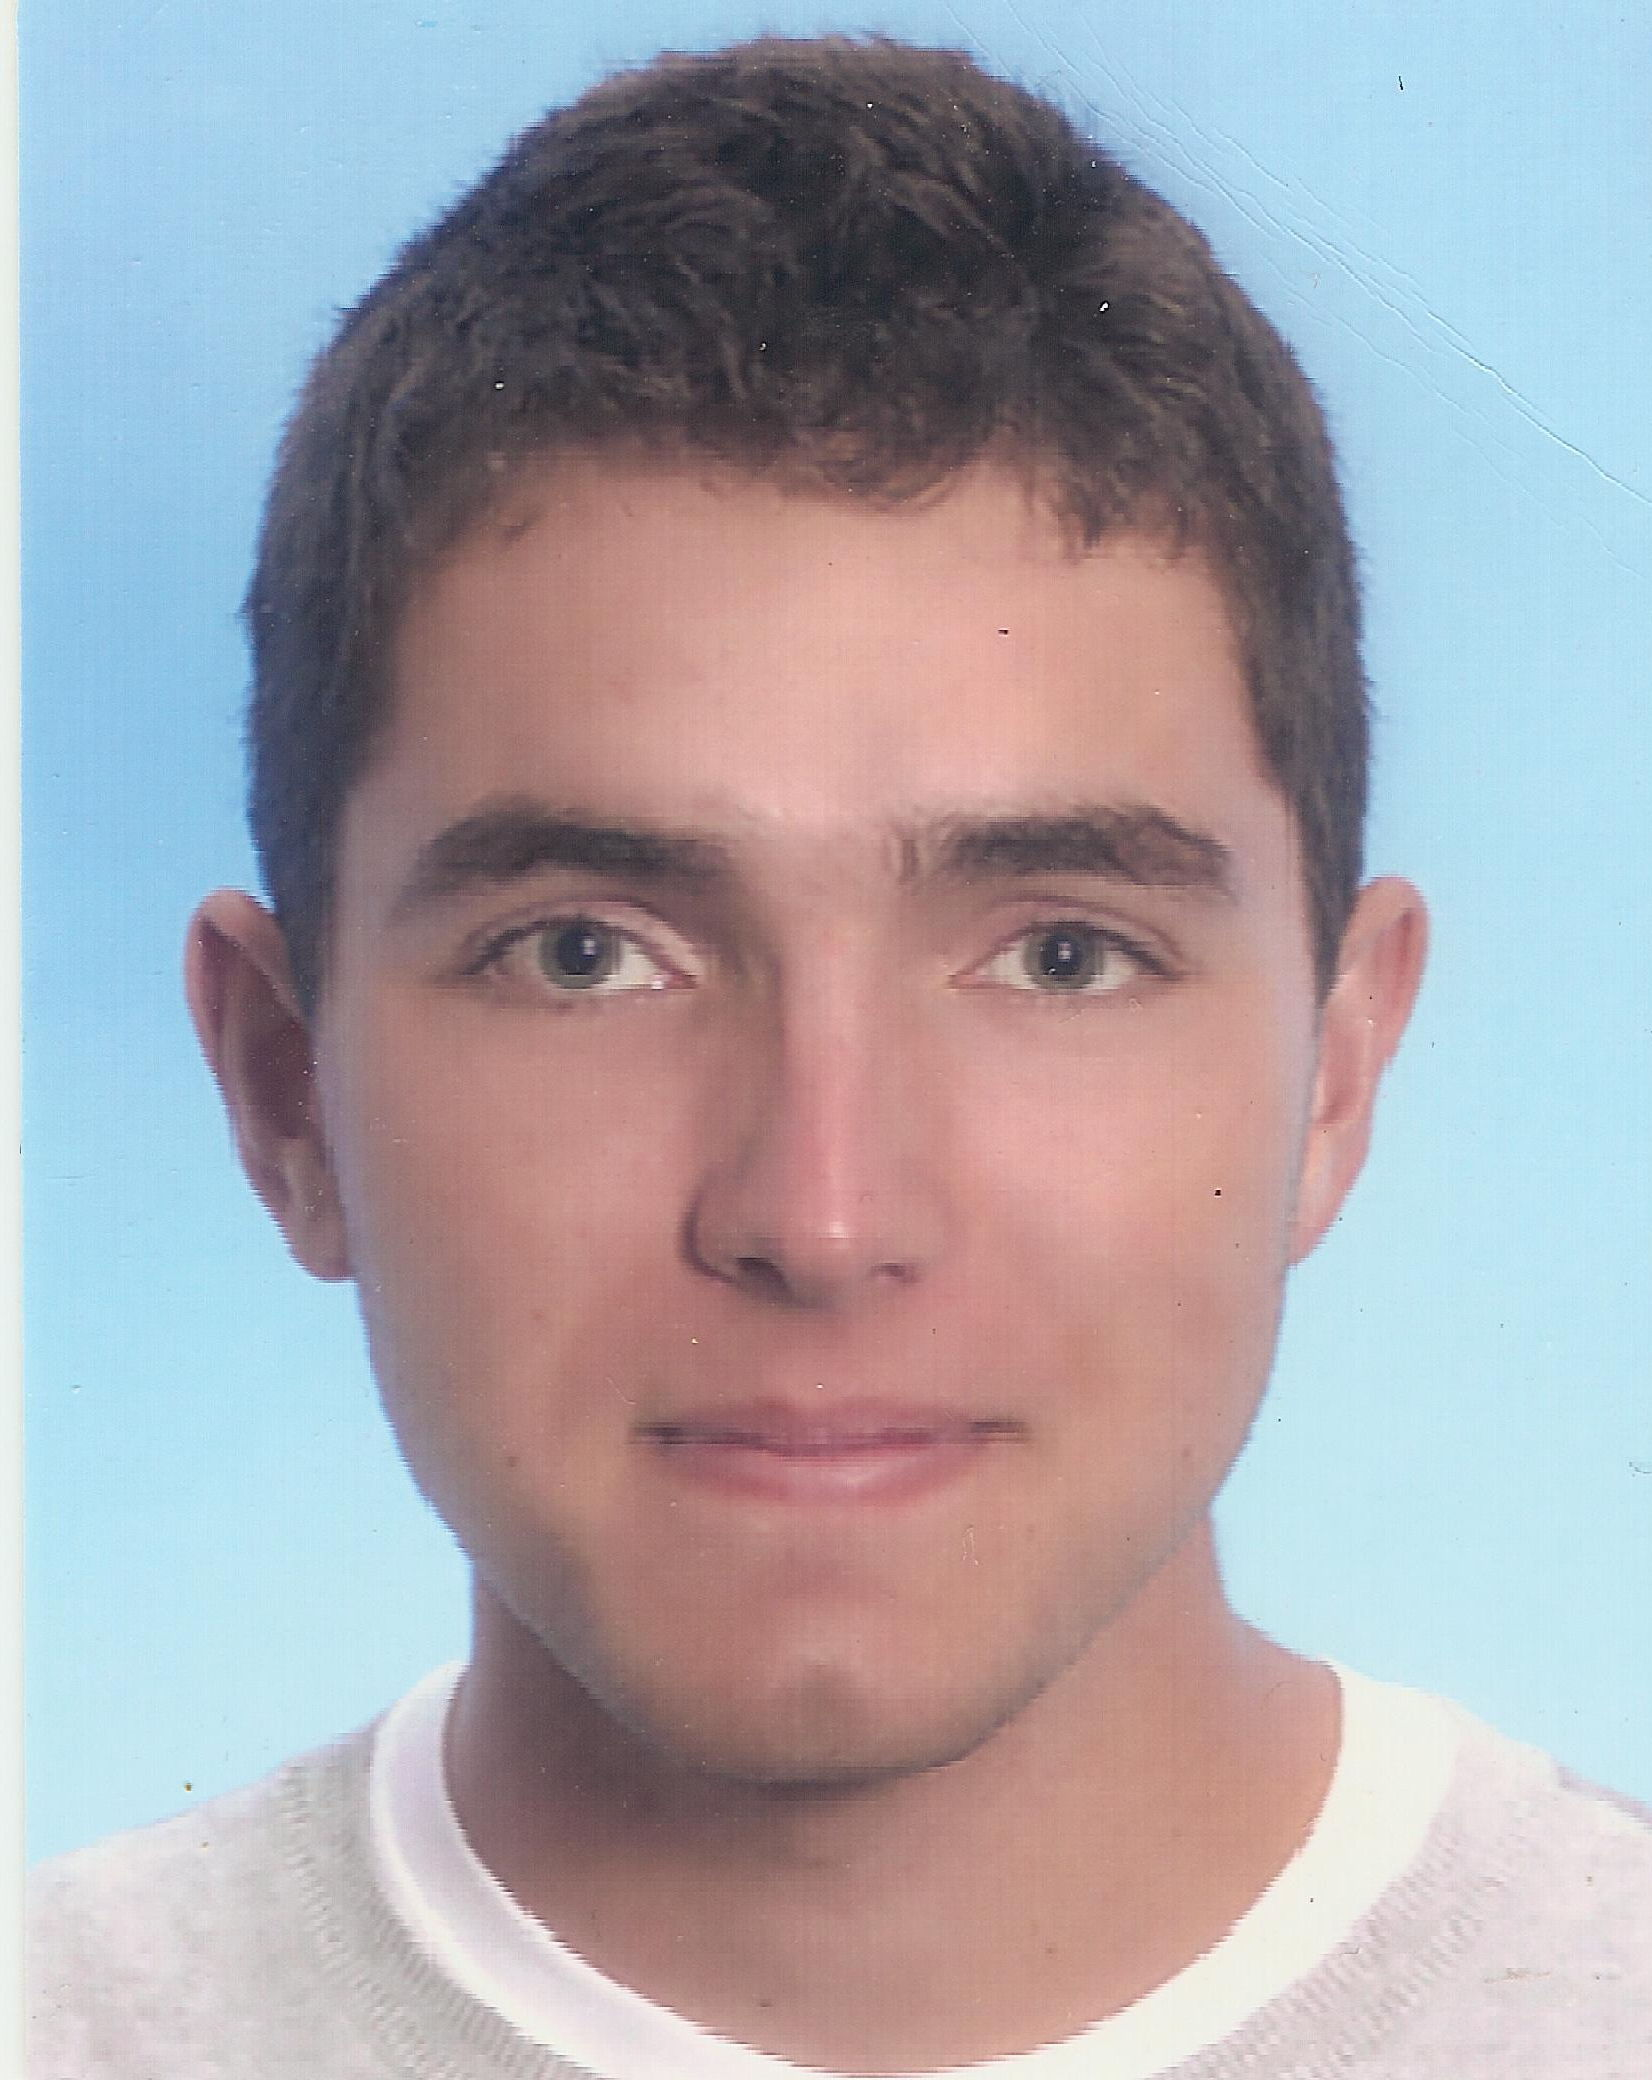
\includegraphics[scale=0.5]{OndrejBlazek.jpg} 
  %\includegraphics[scale=0.02]{PetraOnco.JPG} 
  \end{center}
% Print the footer with 3 arguments(<left>, <center>, <right>)
% Leave any of these blank if they are not needed
\makecvfooter
  {\today}
  {Ondřej Blažek~~~·~~~Curriculum Vitae}
  %{*Dle CEFR.}
  {*According to CEFR.}
  %{\thepage}


%----------------------Type name of new folder---------------------------------------------------------
%	CV/RESUME CONTENT
%	Each section is imported separately, open each file in turn to modify content
%-------------------------------------------------------------------------------
\cvsection{Education}


%-------------------------------------------------------------------------------
%	CONTENT
%-------------------------------------------------------------------------------
\begin{cventries}

%---------------------------------------------------------
  \cventry
    {Brno University of Technology - Faculty of Electrical Engineering and Communication.}
    {Brno}
    {2014 - PRESENT}
    {}
  \cventry
    {Studying abroad - Computer Science}
    {Graz University of Technology}
    {Graz}
    {September 2015 - February 2016}
    {}
  \cventry
    {Bachelor's study - Teleinformatics} % Degree
    {Brno University of Technology - Faculty of Electrical Engineering and Communication.} % Institution
    {Brno} % Location
    {2011 - 2014} % Date(s)
    {}

%---------------------------------------------------------
\end{cventries}

%-------------------------------------------------------------------------------
%	SECTION TITLE
%-------------------------------------------------------------------------------
\cvsection{Skills}
%-------------------------------------------------------------------------------
%	CONTENT
%-------------------------------------------------------------------------------
\begin{cvskills}

%---------------------------------------------------------
  \vspace{5pt}
  
  \cvskill
    {Programming/Scripting} % Category
    {Bash, Python, C, Qt, C++, Visual Basic (vba), Basics of Java} % Skills
%---------------------------------------------------------    
  \vspace{5pt}
  \cvskill
    {Web} % Category
    {HTML, CSS, JavaScript, JQuery \newline Knowledge of revision control systems GIT, SVN}

%---------------------------------------------------------
  \vspace{5pt}
    
  \cvskill
    {Network administration} % Category
    {Knowledge of Cisco IOS - completed courses CCNA, CCNP(Routing) - protocols RIP, OSPF, EIGRP, BGP and \newline experience with VLAN, ACL, Firewalls configuration...\newline RouterOS - Mikrotik} % Skills
%---------------------------------------------------------
  
  \vspace{5pt}
  \cvskill
    {OS}
    {Knowledge of OS Linux (Debian/Ubuntu) - orientation in shell, basic administration, installation \newline Knowledge of OS Windows}
  \vspace{5pt}
    
  \cvskill
    {Foreign languages*} % Category
    {English - C1, German - A2, Swedish - A1} % Skills

%---------------------------------------------------------
\end{cvskills}

%%-------------------------------------------------------------------------------
%	SECTION TITLE
%-------------------------------------------------------------------------------
\cvsection{Ostatní znalosti}


%-------------------------------------------------------------------------------
%	CONTENT
%-------------------------------------------------------------------------------
\begin{cvskills}

  
%---------------------------------------------------------
 \vspace{1pt}
  \cvskill
    {Cizí jazyky} % Category
    {Angličtina - B2/aktivní\newline Francouzština - A1/pasivní} % Skills

%---------------------------------------------------------
\end{cvskills}

%-------------------------------------------------------------------------------
%	SECTION TITLE
%-------------------------------------------------------------------------------
\cvsection{Experiences}


%-------------------------------------------------------------------------------
%	CONTENT
%-------------------------------------------------------------------------------
\begin{cventries}

%---------------------------------------------------------
  \cventry
    {SW Developer Internship}
    {Tieto Czech Support Services s.r.o.}
    {Brno}
    {July 2016 - Present}
    {
      \begin{cvitems}
       \item {Getting to know OpenStack - virtualization technology and OpenDaylight - software defined networking.}
       \item {Working on integration between these two along with OpenvSwitch and DPDK.}
       \item {Exploring features (mininet - Python, Virtual Tenant Network - REST \dots) of OpenDaylight and making automatization scripts using bash.}
      \end{cvitems}
    }
  \cventry
    {NOC operator} % Job title
    {GiTy, a.s.} % Organization
    {Brno} % Location
    {April 2014 - June 2015} % Date(s)
    {
      \begin{cvitems} % Description(s) of tasks/responsibilities
	\item {Technical supervision of MPLS network, satellite network (VSAT) iDirect and Hughes.}
        \item {Contact with a customer and managing of unexpected incidents on the network, potential change in configuration of the network on Mikrotik/Cisco devices.}     
        \item {Network behaviour analysis, including modelling with tool SNMPc and using network monitoring program PRTG.}     
        \item {Processing of customer's demands in system helpdesk or creating SLA reports using vba macros.}        
      \end{cvitems}
    }
   \cventry
   {IT Technician}
   {Zabezpečovací systémy a sítě Studený}
   {Říčany u Brna}
   {November 2013}
   {
    \begin{cvitems}
      \item {Building up LAN infrastructure, adding a network rack.}
    \end{cvitems}
   }
   \cventry
   {IT Technician}
   {Komply.cz}
   {Brno}
   {May 2013}
   {
    \begin{cvitems}
      \item {Building up LAN infrastructure; computer configuration, maintanance.}
    \end{cvitems}
   }
   \cventry
   {Practical training}
   {GiTy, a.s.}
   {Brno}
   {March 2013 - May 2013}
   {
    \begin{cvitems}
      \item {Getting familiar with company's data services, terrestrial and satellite services. Work on a supervision center and it's technical support.}
      \item {Work related to G-Net network node modernization. Switching of the data lines or expansion of the network devices by adding additional modules and their configuration.}
    \end{cvitems}
   }
   
   \cventry
   {Practical training}
   {ABA Czech, s.r.o.}
   {Hustopeče}
   {2010}
   {
    \begin{cvitems}
      \item {Getting to know system Novell, reinstallation of computers with OS Microsoft Windows.}
    \end{cvitems}
   }

%---------------------------------------------------------
\end{cventries}

%-------------------------------------------------------------------------------
%	SECTION TITLE
%-------------------------------------------------------------------------------
\vspace{1.5cm}
\cvsection{Ostatní informace}

\cvsubsection{Kurzy}


%-------------------------------------------------------------------------------
%	CONTENT
%-------------------------------------------------------------------------------
\begin{cvhonors}

%---------------------------------------------------------
  \cvhonor
    {}% Award
    {Seminář Beton University 2014} % Event
    % Location
    % Date(s)



%---------------------------------------------------------
\end{cvhonors}
\vspace{5pt}
\cvsubsection{Licence}


%-------------------------------------------------------------------------------
%	CONTENT
%-------------------------------------------------------------------------------
\begin{cvhonors}

%---------------------------------------------------------
  \cvhonor
    {}% Award
    {Řidičský průkaz: Skupina B} % Event
    % Location
    % Date(s)



%---------------------------------------------------------
\end{cvhonors}
\vspace{5pt}
\cvsubsection{Vlastnosti}


%-------------------------------------------------------------------------------
%	CONTENT
%-------------------------------------------------------------------------------
\begin{cvhonors}

%---------------------------------------------------------
  \cvhonor
    {} % Award
    {Flexibilita, entuziasmus, přijemné vystupování, pečlivost.} % Event
     % Location
     % Date(s)

%---------------------------------------------------------
\end{cvhonors}
\vspace{5pt}
%-------------------------------------------------------------------------------
%	SUBSECTION TITLE
%-------------------------------------------------------------------------------
\cvsubsection{Zájmy}


%-------------------------------------------------------------------------------
%	CONTENT
%-------------------------------------------------------------------------------
\begin{cvhonors}

%---------------------------------------------------------
  \cvhonor
    {} % Award
    {Cestování, četba, fotografování, kresba, kultura, sport (rekreačně volejbal, lyžování, jízda na kole).} % Event
     % Location
     % Date(s)

%---------------------------------------------------------
\end{cvhonors}
\vspace{5pt}



%%-------------------------------------------------------------------------------
%	SECTION TITLE
%-------------------------------------------------------------------------------
\cvsection{Extracurricular Activity}


%-------------------------------------------------------------------------------
%	CONTENT
%-------------------------------------------------------------------------------
\begin{cventries}

%---------------------------------------------------------
  \cventry
    {Core Member} % Affiliation/role
    {B10S (B1t 0n the Security, Underground hacker team)} % Organization/group
    {S.Korea} % Location
    {Nov. 2011 - PRESENT} % Date(s)
    {
      \begin{cvitems} % Description(s) of experience/contributions/knowledge
        \item {Gained expertise in penetration testing areas, especially targeted on web application and software.}
        \item {Participated on a lot of hacking competition and won a good award.}
        \item {Held several hacking competitions non-profit, just for fun.}
      \end{cvitems}
    }

%---------------------------------------------------------
  \cventry
    {Member} % Affiliation/role
    {WiseGuys (Hacking \& Security research group)} % Organization/group
    {S.Korea} % Location
    {Jun. 2012 - PRESENT} % Date(s)
    {
      \begin{cvitems} % Description(s) of experience/contributions/knowledge
        \item {Gained expertise in hardware hacking areas from penetration testing on several devices including wireless router, smartphone, CCTV and set-top box.}
        \item {Trained wannabe hacker about hacking technique from basic to advanced and ethics for white hackers by hosting annual Hacking Camp.}
      \end{cvitems}
    }

%---------------------------------------------------------
  \cventry
    {Core Member \& President at 2013} % Affiliation/role
    {PoApper (Developers' Network of POSTECH)} % Organization/group
    {Pohang, S.Korea} % Location
    {Jun. 2010 - PRESENT} % Date(s)
    {
      \begin{cvitems} % Description(s) of experience/contributions/knowledge
        \item {Reformed the society focusing on software engineering and building network on and off campus.}
        \item {Proposed various marketing and network activities to raise awareness.}
      \end{cvitems}
    }

%---------------------------------------------------------
  \cventry
    {Member} % Affiliation/role
    {PLUS (Laboratory for UNIX Security in POSTECH)} % Organization/group
    {Pohang, S.Korea} % Location
    {Sep. 2010 - Oct. 2011} % Date(s)
    {
      \begin{cvitems} % Description(s) of experience/contributions/knowledge
        \item {Gained expertise in hacking \& security areas, especially about internal of operating system based on UNIX and several exploit techniques.}
        \item {Participated on several hacking competition and won a good award.}
        \item {Conducted periodic security checks on overall IT system as a member of POSTECH CERT.}
        \item {Conducted penetration testing commissioned by national agency and corporation.}
      \end{cvitems}
    }

%---------------------------------------------------------
  \cventry
    {Member} % Affiliation/role
    {MSSA (Management Strategy Club of POSTECH)} % Organization/group
    {Pohang, S.Korea} % Location
    {Sep. 2013 - PRESENT} % Date(s)
    {
      \begin{cvitems} % Description(s) of experience/contributions/knowledge
        \item {Gained knowledge about several business field like Management, Strategy, Financial and marketing from group study.}
        \item {Gained expertise in business strategy areas and inisght for various industry from weekly industry analysis session.}
      \end{cvitems}
    }

%---------------------------------------------------------
\end{cventries}

%%-------------------------------------------------------------------------------
%	SECTION TITLE
%-------------------------------------------------------------------------------
\cvsection{Presentation}


%-------------------------------------------------------------------------------
%	CONTENT
%-------------------------------------------------------------------------------
\begin{cventries}

%---------------------------------------------------------
  \cventry
    {Presenter for <DEFCON 20th : The way to go to Las Vegas>} % Role
    {6th CodeEngn (Reverse Engineering Conference)} % Event
    {Seoul, S.Korea} % Location
    {Jul. 2012} % Date(s)
    {
      \begin{cvitems} % Description(s)
        \item {Introduced CTF(Capture the Flag) hacking competition and advanced techniques and strategy for CTF}
      \end{cvitems}
    }

%---------------------------------------------------------
  \cventry
    {Presenter for <Metasploit 101>} % Role
    {6th Hacking Camp - S.Korea} % Event
    {S.Korea} % Location
    {Sep. 2012} % Date(s)
    {
      \begin{cvitems} % Description(s)
        \item {Introduced basic procedure for penetration testing and how to use Metasploit}
      \end{cvitems}
    }

%---------------------------------------------------------
\end{cventries}

%%-------------------------------------------------------------------------------
%	SECTION TITLE
%-------------------------------------------------------------------------------
\cvsection{Writing}


%-------------------------------------------------------------------------------
%	CONTENT
%-------------------------------------------------------------------------------
\begin{cventries}

%---------------------------------------------------------
  \cventry
    {Founder \& Writer} % Role
    {A Guide for Developers in Start-up} % Title
    {Facebook Page} % Location
    {Jan. 2015 - PRESENT} % Date(s)
    {
      \begin{cvitems} % Description(s)
        \item {Drafted daily news for developers in Korea about IT technologies, issues about start-up.}
      \end{cvitems}
    }

%---------------------------------------------------------
  \cventry
    {Undergraduate Student Reporter} % Role
    {AhnLab} % Title
    {S.Korea} % Location
    {Oct. 2012 - Jul. 2013} % Date(s)
    {
      \begin{cvitems} % Description(s)
        \item {Drafted reports about IT trends and Security issues on AhnLab Company magazine.}
      \end{cvitems}
    }

%---------------------------------------------------------
\end{cventries}

%%-------------------------------------------------------------------------------
%	SECTION TITLE
%-------------------------------------------------------------------------------
\cvsection{Program Committees}


%-------------------------------------------------------------------------------
%	CONTENT
%-------------------------------------------------------------------------------
\begin{cvhonors}

%---------------------------------------------------------
  \cvhonor
    {Problem Writer} % Position
    {2016 CODEGATE Hacking Competition World Final} % Committee
    {S.Korea} % Location
    {2016} % Date(s)

%---------------------------------------------------------
  \cvhonor
    {Organizer \& Co-director} % Position
    {1st POSTECH Hackathon} % Committee
    {S.Korea} % Location
    {2013} % Date(s)

%---------------------------------------------------------
  \cvhonor
    {Staff} % Position
    {7th Hacking Camp} % Committee
    {S.Korea} % Location
    {2012} % Date(s)

%---------------------------------------------------------
  \cvhonor
    {Problem Writer} % Position
    {1st Hoseo University Teenager Hacking Competition} % Committee
    {S.Korea} % Location
    {2012} % Date(s)

%---------------------------------------------------------
  \cvhonor
    {Staff \& Problem Writer} % Position
    {JFF(Just for Fun) Hacking Competition} % Committee
    {S.Korea} % Location
    {2012} % Date(s)

%---------------------------------------------------------
\end{cvhonors}



%-------------------------------------------------------------------------------
\end{document}
